\chapter{Current state}
\label{ch:currentState}

\section{About convolutional neural networks}

The model that is used for this project is from the family of convolutional neural networks or CNNs. These are models that are especially useful to perform operations on digital images. CNNs contain at least one convolutional layer that computes a mathematical operation that is called discrete convolution. Discrete convolution operation has been proved useful when applied on digital images to detect structural features like edges and corners.

The advantage of CNNs compared to traditional multi layer perceptrons (MLPs) is that discrete convolutional operation is translational invariant. This means it is irrelevant where in a given image a specific object is located: The model will not learn the position of the specific object. Another huge advantage of CNNs over MLPs is that CNNs usually have sparse interactions. This means that it is possible to yield a good performance even if some adjacent layers are not fully connected with each other. Another way to speed up the training process is to use parameter sharing: Some weigths will be used at multiple places at the same time. These two techniques, sparse interactions and parameter sharing does make it possible to train very deep neural networks in a feasible time.

When applying discrete convolution to an image, a filter with a given kernel is used to perform convolution on the image. To detect edges and corners there exist specific kernels especially for that kind of purpose. But often it is also possible to learn the optimal kernel in the process of machine learning.

Another important kind of layer that is usually employed in CNNs are pooling layers. Also called subsampling or downsampling layers sometimes, they reduce the size of a given image. Some frequently used pooling layers are max- and average-pooling. The advantages of pooling layers are smaller input, parameter reduction and more invariance to scaling and transformations.

The third important kind of layer is ReLU (rectified linear unit). The mere us of this layer is to preprocess the image before the next convolutional operation. This just adjusts the image brightness in a ways that all negative values (values that are darker than the middle grey of an image) got adjusted to middle grey.

\section{From CNNs to Mask R-CNN}

The very first CNN  appeared in the year 1994, it was named LeNet5, by Yann LeCun. This fundamental work was the first network that used convolutional and pooling layers to process images. In a time long before consumer graphic processing units (GPUs), where even CPUs were slow, it was important to reduce the number of parameters to a bare minimum (accomplished with sparse connect layers).

Starting with AlexNet by Alex Krizhevsky, Ilya Sutskever and Geoffrey Hinton in 2012, CNNs gained significantly performance gains when applied on image classification tasks. AlexNet took the idea of a CNN from LeNet5 and added more layers to it and was the first to include ReLU layers. It also used dropout techniques to avoid overfitting during the training process. AlexNet was still an image detection model, trained to label images. This means a single label (class) is given to a whole input image.

ResNet (residual neural network) in 2015 was the first CNN that included residual blocks or identity shortcut connections. This are connections in the network that skip one or more layers and just use the input value as an output (mathematical identity). This was another step to reduce computation cost and lead to even deeper networks. ResNet is still used today as part of the backbone in a lot of object detection and instance segmentation models.

With R-CNN (regions with CNN features) in 2013, the rise of object detection models began. These researcher asked themself, how can one use the technique from CNNs to not only classify an image but to classify objects in that image?  These family of models are capable of labelling multiple objects depicted in the same image with each a bounding box and a class prediction. R-CNN models do that by proposing regions in that potential objects may lie. R-CNN is thus called a two stage model: The first stage scans the image and generates region proposals, whereas the second stage uses these regions to extract CNN features from it and to ultimately classify objects in it. For the classification step in the last layer, R-CNN uses a support vector machine (SVM) as a classifier. In the very last step, a regression is used to further tighten the coordinates of the bounding boxes of each object.

\begin{figure}[!h]
	\center{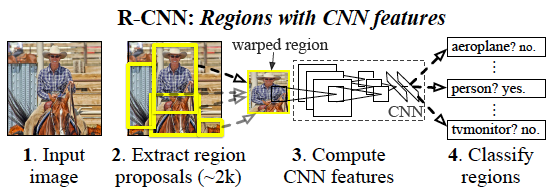
\includegraphics[width=350pt]
	{img/r-cnn.png}}
	\caption{\label{fig:input-image} Architecture of R-CNN}
\end{figure}

In 2017, the team from Ross Girshick, one of the creators of R-CNN, delivered Fast R-CNN an improved, faster version of it. In R-CNN there are a lot of overlapping region proposals and every computation gets calculated again, even if the regions are very similar to each other. To circumvent this he invented region of interest pooling (RoIPool). RoIPool shares these computation across the regions of an image and can speed up computation a lot. The other improvement was to put all computation in a single network (compared to R-CNN where for example classification ran in a single network).

Also in 2017, also by the team from Ross Girshik, the second iteration of R-CNN got released, called Faster R-CNN. The main improvement was to use just one CNN that produces a feature map for both region proposal and classification.

With Mask R-CNN from 2017 (also by Ross Girshik et. al) it is also possible to not only predict the bounding box of an object but also to predict a mask that shows the exact shape of the object (called pixel level segmentation). These models are called instance segmentation models. This is accomplished by adding a branch to the model that computes a binary mask for a given object in the image. Mask R-CNN model is of the family of object or instance segmentation models.

An overview over the different tasks and approaches and their models  in the field of object recognition can be seen here:

\begin{figure}[!h]
	\center{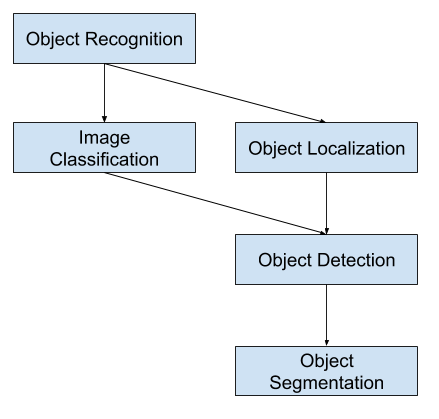
\includegraphics[width=350pt]
	{img/object-recognition.png}}
	\caption{\label{fig:input-image} Tasks and approaches in object recognition}
\end{figure}

